\documentclass{article}

\usepackage{qa}

\begin{document}

\customtitle{Homework 6}
\customauthor{Hamza Kamal}
\customdate{\today}

\qna {
    Q1. (6 points) A full-adder is a combinational circuit that forms the arithmetic sum of three input bits. It consists of three inputs, x, y, z, and two outputs, C and S. Two of the input, that is, x and y, represent the two significant bits to be added. The third input, z, represents the carry from the previous lower significant position. The output S denotes the sum of two bits and C denotes carry. Answer the following sub-questions. \\
    a. Construct a truth table for the Full-Adder
} {
    Truth Table: \\
    \linebreak
    \begin{tabular}{|c | c | c | c | c |}
        \hline
        x & y & z & C & S \\
        \hline
        0 & 0 & 0 & 0 & 0 \\
        \hline
        0 & 0 & 1 & 1 & 0 \\
        \hline
        0 & 1 & 0 & 1 & 0 \\
        \hline
        0 & 1 & 1 & 0 & 1 \\
        \hline
        1 & 0 & 0 & 1 & 0 \\
        \hline
        1 & 0 & 1 & 0 & 1 \\
        \hline
        1 & 1 & 0 & 0 & 1 \\
        \hline
        1 & 1 & 1 & 1 & 1 \\
        \hline
    \end{tabular}
}

\qna {
    b. Based on the truth table, construct a K-map for the output S and derive a Boolean equation using K-map. Make the equation as simple as possible. \\
} {
    S K-map: \\
    \linebreak
    \begin{tabular}{|c|c|c|c|c|}
        \hline
          & 00 & 01 & 11 & 10 \\
        \hline
        0 & 0  & 1  & 0  & 1  \\
        \hline
        1 & 1  & 0  & 1  & 0  \\
        \hline
    \end{tabular} \\
    \linebreak
    S = $\neg x yz + \neg x y \neg z + x \neg y \neg z + xyz$
}

\qna {
    c. Based on the truth table, construct a K-map for the output C and derive a Boolean equation using K-map. Make the equation as simple as possible. \\
} {
    C K-map: \\
    \linebreak
    \begin{tabular}{|c|c|c|c|c|}
        \hline
          & 00 & 01 & 11 & 10 \\
        \hline
        0 & 0  & 0  & 1  & 0  \\
        \hline
        1 & 1  & 1  & 1  & 1  \\
        \hline
    \end{tabular} \\
    \linebreak
    C = $yz + x$
}

\qna {
    d. By algebraic manipulation, show that S can be expressed as the exclusive-OR of the three input variables. That is, show that, \\
    $S = x \oplus y \oplus z$ \\
} {
    \[
        S = x \oplus y \oplus z = (x \oplus y) \oplus z
    \]

    \[
        x \oplus y = \neg x y + x \neg y, \quad (x \oplus y) \oplus z = (\neg x y + x \neg y) \oplus z
    \]

    \[
        = \neg (\neg x y + x \neg y) z + (\neg x y + x \neg y) \neg z
    \]

    \[
        = \neg (x \neg y + \neg x \neg y) z + (\neg x y + x \neg y) \neg z
    \]

    \[
        = (\neg x y + x y) z + (\neg x y + x \neg y) \neg z
    \]

    \[
        = \neg x y z + x y z + \neg x y \neg z + x \neg y \neg z
    \]

    \[
        = \neg x \neg y z + \neg x y \neg z + x \neg y \neg z + x y z
    \]
}

\qna {
    e.  By algebraic manipulation, show that C can be expressed as the following term. \\
    $C = xy + (x \oplus y) z$ \\
} {
    \[
        = xy + (\neg x y + x \neg y)z = xy + \neg x y z + x \neg y z
    \]

    \[
        xy + \neg x y z + x \neg y z = xy + \neg x y z + x \neg y z
    \]

    \[
        = xy + yz (\neg x) + xz (\neg y)
    \]

    \[
        = xy + yz - xy z + xz - xy z
    \]

    \[
        = xy + yz + xz - 2xy z
    \]

    \[
        = xy + yz + xz - xy z - xy z
    \]

    \[
        = xy(1 - z) + yz + xz - xy z
    \]

    \[
        = xy - xy z + yz + xz - xy z
    \]

    \[
        = xy + yz + xz - 2xy z
    \]

    \[
        = xy + yz + xz
    \]

    \[
        = yz + xz + xy
    \]
    \[
        = yz + x
    \]
}

\qna {
    Based on d and e, draw a circuit for the full-adder in Logisim simulator, attach the image file and submit the circuit file! \\
} {
    sup
}

\qna {
    Q2. (4 points) A sequential circuit has one D flip-flop and one JK flip-flop, two inputs x and y, and one output z. A is the output of D flip-flop, and B is the output of JK-flip-flop; A and B together form the "output state" of the circuit. The flip-flop input equations and the circuit output are as follows. Here DA is the D input of the D-flip flop of A, and JB, KB is the J and K input of the JK-flip flop of B. \\
    \[
        DA = \neg x y + y B
    \]

    \[
        JB = \neg y B + x y
    \]

    \[
        KB = x B + \neg y A
    \]

    \[
        z = x + \neg x y
    \] \\
    a. Draw the logic diagram of the circuit and test it with Logisim. \\
    Please attach the circuit image and the generated table! \\
} {
    Generated Table: \\
    \linebreak
    \begin{tabular}{|c|c|c|}
        \hline
        x & y & z \\
        \hline
        0 & 0 & 1 \\
        \hline
        0 & 1 & 1 \\
        \hline
        1 & 0 & 0 \\
        \hline
        1 & 1 & 0 \\
        \hline
    \end{tabular}
}

\qna {
    b. Construct a state diagram of this circuit. \\
} {
    $$
        A_{n+1} = D_A = \sim xy + yB_n
    $$

    $$
        B_{n+1} = J_B \sim B_n + K_B B_n = (\sim y B_n + xy) \sim B_n + (x B_n + (\sim y) A_n) B_n
    $$

    $$
        = \sim y B_n \sim B_n + xy \sim B_n + x B_n B_n + \sim y A_n B_n
    $$

    $$
        = 0 + xy \sim B_n + x B_n + \sim y A_n B_n
    $$

    $$
        B_{n+1} = xy \sim B_n + x B_n + \sim y A_n B_n
    $$

    $$
        z = x + \sim xy
    $$ \\
    State Table: \\
    \linebreak
    \begin{tabular}{|c|c|c|c|c|}
        \hline
        Input & Present State & Next State        & Output \\
        \hline
        xy    & $A_n B_n$     & $A_{n+1} B_{n+1}$ & z      \\
        \hline
        00    & 00            & 00                & 0      \\
        \hline
        00    & 01            & 00                & 0      \\
        \hline
        00    & 10            & 00                & 0      \\
        \hline
        00    & 11            & 01                & 0      \\
        \hline
        01    & 00            & 10                & 1      \\
        \hline
        01    & 01            & 10                & 1      \\
        \hline
        01    & 10            & 10                & 1      \\
        \hline
        01    & 11            & 10                & 1      \\
        \hline
        10    & 00            & 00                & 1      \\
        \hline
        10    & 01            & 01                & 1      \\
        \hline
        10    & 10            & 00                & 1      \\
        \hline
        10    & 11            & 01                & 1      \\
        \hline
        11    & 00            & 01                & 1      \\
        \hline
        11    & 01            & 11                & 1      \\
        \hline
        11    & 10            & 01                & 1      \\
        \hline
        11    & 11            & 11                & 1      \\
        \hline
    \end{tabular} \\
    \linebreak
    \begin{figure}[H]
        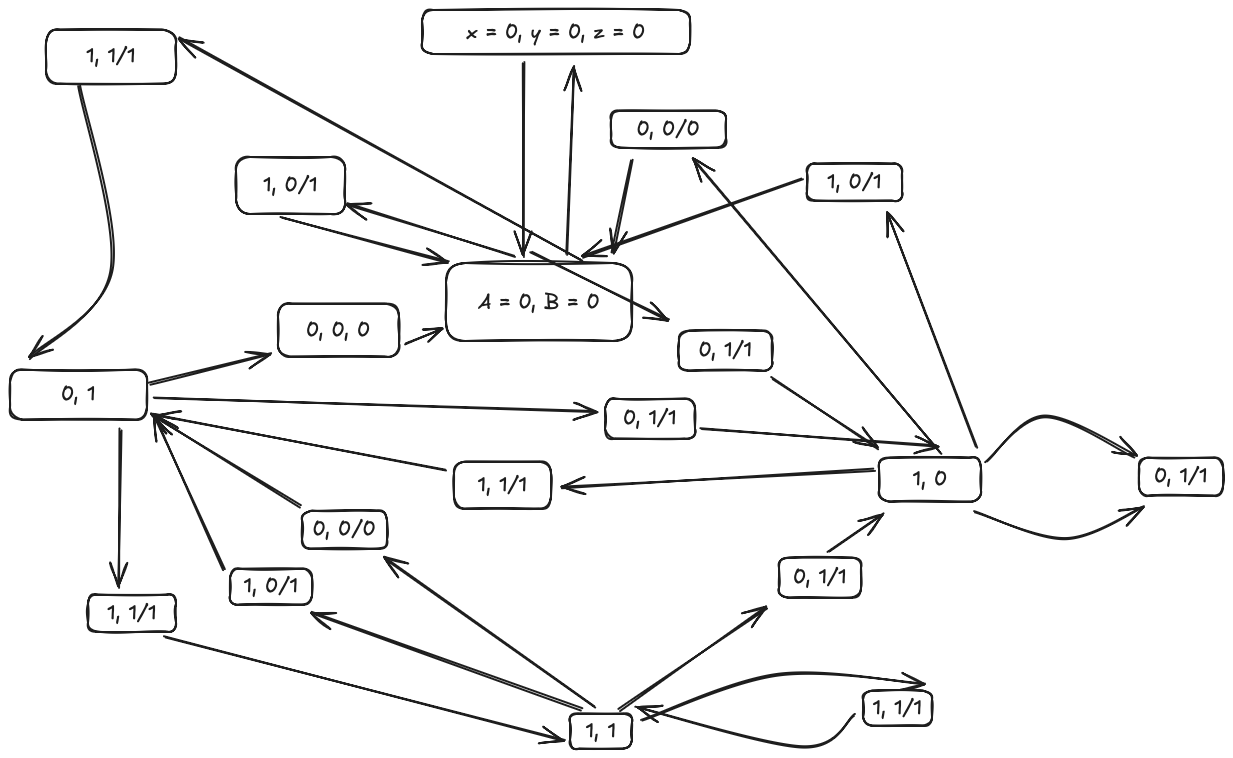
\includegraphics[width=\textwidth]{./img/Q2-State-Diagram.png}
    \end{figure}
}

\qna {
    Q3. (10 points) Design a system with the following state changes: This is a sequential circuit with three flip-flops. The state sequence is changed with a clock as in the order of, 111, 010, 100,110, 001, 011, 101, 000, 111 and repeat. Use JK flip-flops. \\
    a. Draw a state diagram. \\
} {
    \begin{figure}[H]
        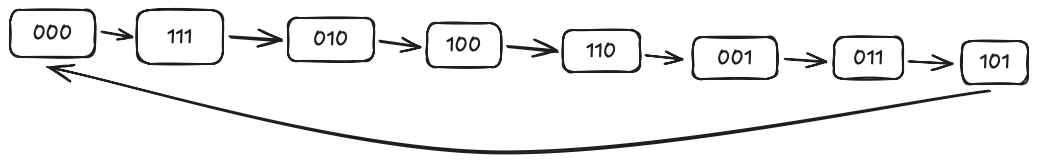
\includegraphics[width=\textwidth]{./img/Q3-State-Diagram.png}
    \end{figure}
}

\qna {
    b. Construct an excitation table. \\
} {
    \begin{tabular}{|c|c|c|c|c|c|c|c|}
        \hline
        Present State & Next State  & Flip Flop Inputs &    &    &    &    &    \\
        \hline
        Q2 Q1 Q0      & Q2+ Q1+ Q0+ & J2               & K2 & J1 & K1 & J0 & K0 \\
        \hline
        111           & 010         & 0                & 1  & 0  & 0  & 0  & 1  \\
        \hline
        010           & 100         & 1                & X  & 0  & 1  & 0  & X  \\
        \hline
        100           & 110         & 0                & 0  & 1  & X  & 0  & X  \\
        \hline
        110           & 001         & 0                & 1  & 0  & 1  & 1  & X  \\
        \hline
        001           & 011         & 0                & X  & 1  & X  & 0  & 0  \\
        \hline
        011           & 101         & 1                & X  & 0  & 1  & 0  & 0  \\
        \hline
        101           & 000         & 0                & 1  & 0  & X  & 0  & 1  \\
        \hline
        000           & 111         & 1                & X  & 1  & X  & 1  & X  \\
        \hline
    \end{tabular}
}

\qna {
    c. Draw K-maps and derive Boolean equations using K-maps. Make the equations as simple as possible. \\
} {
    J0 K-map: \\
    \begin{tabular}{|c|c|c|c|c|}
        \hline
          & 00 & 01 & 11 & 10 \\
        \hline
        0 & 1  & 0  & X  & X  \\
        \hline
        1 & X  & X  & 0  & 1  \\
        \hline
    \end{tabular} \\
    \linebreak
    J1 K-map: \\
    \begin{tabular}{|c|c|c|c|c|}
        \hline
          & 00 & 01 & 11 & 10 \\
        \hline
        0 & 1  & 1  & 0  & X  \\
        \hline
        1 & X  & X  & 0  & 1  \\
        \hline
    \end{tabular} \\
    \linebreak
    J2 K-map: \\
    \begin{tabular}{|c|c|c|c|c|}
        \hline
          & 00 & 01 & 11 & 10 \\
        \hline
        0 & 1  & 1  & 0  & 1  \\
        \hline
        1 & X  & X  & 0  & 0  \\
        \hline
    \end{tabular} \\
    \linebreak
    K0 K-map: \\
    \begin{tabular}{|c|c|c|c|c|}
        \hline
          & 00 & 01 & 11 & 10 \\
        \hline
        0 & 1  & 0  & X  & X  \\
        \hline
        1 & X  & X  & 0  & 1  \\
        \hline
    \end{tabular} \\
    \linebreak
    K1 K-map: \\
    \begin{tabular}{|c|c|c|c|c|}
        \hline
          & 00 & 01 & 11 & 10 \\
        \hline
        0 & X  & X  & X  & 1  \\
        \hline
        1 & X  & X  & 1  & 1  \\
        \hline
    \end{tabular} \\
    \linebreak
    K2 K-map: \\
    \begin{tabular}{|c|c|c|c|c|}
        \hline
          & 00 & 01 & 11 & 10 \\
        \hline
        0 & X  & X  & X  & X  \\
        \hline
        1 & X  & 1  & 1  & 1  \\
        \hline
    \end{tabular} \\
    $J_0 = \neg Q_2 \neg Q_1 \neg Q_0 + Q_2 Q_1 \neg Q_0$                                                      \\
    $= \neg Q_0 (\neg Q_2 \neg Q_1 + Q_2 Q_1)$                                                                 \\
    $J_1 = \neg Q_2 \neg Q_1 \neg Q_0 + \neg Q_2 \neg Q_1 Q_0 + Q_2 \neg Q_1 \neg Q_0$                         \\
    $= \neg Q_1 (\neg Q_0 + \neg Q_2 Q_0) + Q_2 \neg Q_1 \neg Q_0 = \neg Q_1 \neg Q_0 + \neg Q_1 \neg Q_2 Q_0$ \\
    $J_2 = \neg Q_2 \neg Q_1 \neg Q_0 + \neg Q_2 \neg Q_1 Q_0 + \neg Q_2 Q_1 Q_0$                              \\
    $= \neg Q_2(\neg Q_1 + Q_1 Q_0)$                                                                           \\
    $K_0 = Q_2 Q_0 + Q_2 Q_1$                                                                                  \\
    $K_1 = Q_1 (Q_2 + Q_0)$                                                                                    \\
    $K_2 = Q_2$                                                                                                \\
}

\qna {
    e. Draw the system in Logisim simulator, attach the circuit image and submit the circuit file. \\
    f. Test the system and attach the generated table. \\
} {
    sup
}

\end{document}